\documentclass[a4paper,12pt]{article}
\usepackage{geometry}
\usepackage{wrapfig}
\geometry{
	a4paper,
	total={170mm,257mm},
	left=10mm,
	right=10mm,
	top=20mm,
}
\usepackage{titlesec}
\titlelabel{\thetitle.\quad} %точка в section

%%% Работа с русским языком
\usepackage{cmap}                           % поиск в PDF
\usepackage{mathtext} 			 	       % русские буквы в формулах
\usepackage[T2A]{fontenc}               % кодировка
\usepackage[utf8]{inputenc}              % кодировка исходного текста
\usepackage[english,russian]{babel}  % локализация и переносы

%Математика
\usepackage{amsmath,amsfonts,amssymb,amsthm,mathtools} % AMS
\usepackage{icomma} % "Умная" запятая

%% Шрифты
\usepackage{euscript}	 % Шрифт Евклид
\usepackage{mathrsfs} % Красивый матшрифт

\usepackage{gensymb}
\usepackage{graphicx}
\usepackage{setspace}
\usepackage{tabularx}
\usepackage{longtable}
\usepackage{icomma}
\usepackage{euscript}
\usepackage{float}
\usepackage{cutwin}
\usepackage{adjustbox}
\usepackage{dashbox}
\usepackage[normalem]{ulem}
\usepackage[babel=true]{microtype}
\RequirePackage[T1]{fontenc}
\usepackage{amsmath,amsfonts,amssymb,amsthm,mathrsfs,mathtools}
\usepackage{xcolor}
\usepackage{enumitem}
\usepackage{xpatch}
\usepackage{cancel}
\usepackage{upgreek}
\usepackage{lipsum}
\usepackage[version=4]{mhchem}
\usepackage{multirow}
\usepackage{stackengine}
\usepackage{tikz}
\usepackage{hyperref}
\hypersetup{colorlinks=true,urlcolor=blue}
\usetikzlibrary{positioning}
\usepackage{titletoc}
\usepackage{chngcntr}
\usepackage{fancyhdr}
\usepackage{makecell}
\usepackage{indentfirst}
\usepackage{tocloft}
\usepackage{soul}
\usepackage[stable]{footmisc}
\usepackage{subfig}
\usepackage{comment}


\mathtoolsset{showonlyrefs=true}


\theoremstyle{definition}
\newtheorem*{definition}{Определение}
\newtheorem{statement}{Предложение}[section]
\newtheorem{lemma}{Лемма}[section]
\newtheorem{theorem}{Теорема}[section]
\newtheorem*{theoremn}{Теорема}
\newtheorem*{corollary}{Следствие}
\newtheorem*{example}{Пример}
\newtheorem*{note}{Замечание}
\newtheorem*{problem}{Задача}


\counterwithout{footnote}{section}\DeclareRobustCommand{\divby}{%
	\mathrel{\text{\vbox{\baselineskip.65ex\lineskiplimit0pt\hbox{.}\hbox{.}\hbox{.}}}}%
}

\newcommand{\dotpr}[2]{\bra{#1}\ket{#2}}
\let\AA\relax
\let\emptyset\varnothing
\DeclareMathOperator*{\esssup}{ess sup}
\DeclareMathOperator*{\ord}{ord}
\DeclareMathOperator*{\supp}{supp}
\DeclareMathOperator*{\pr}{pr}
\DeclareMathOperator*{\Ker}{Ker}
\DeclareMathOperator*{\Vol}{Vol}
\DeclareMathOperator*{\rg}{rk}
\DeclareMathOperator*{\Ima}{Im}
\DeclareMathOperator*{\Alt}{Alt}
\DeclareMathOperator*{\Sym}{Sym}
\newcommand{\eqdef}{\stackrel{\text{\tiny{def}}}{=}}
\newcommand{\pp}{\partial}
\newcommand{\AA}{\mathcal{A}}
\newcommand{\BB}{\mathcal{B}}
\newcommand{\MM}{\mathbb{M}}
\newcommand{\NN}{\mathbb{N}}
\newcommand{\ZZ}{\mathbb{Z}}
\newcommand{\QQ}{\mathbb{Q}}
\newcommand{\RR}{\mathbb{R}}
\newcommand{\CC}{\mathbb{C}}
\newcommand{\FFF}{\mathbb{F}}
\newcommand{\DD}{\mathcal{D}}
\newcommand{\FF}{\mathcal{F}}
\newcommand{\sS}{\mathcal{S}}
\newcommand*\circled[1]{\tikz[baseline=(char.base)]{
		\node[shape=circle,draw,inner sep=2pt] (char) {#1};}}

%%% Заголовок
\author{Балдин Виктор Б01-303}
\title{Лабораторная работа 4.1.1 \\
	\textbf{Геометрическая оптика}}
\date{\today}

\begin{document}

{\Large \maketitle}

	\paragraph*{Цель работы:} изучение свойств оптических систем: определение фокусных расстояний линз, определение фокусных расстояний и положения главной и фокальной плоскостей сложной оптической системы, изучение аббераций оптических систем.

	\paragraph*{В работе используются:} оптическая скамья с набором рейтеров, положительные и отрицательные линзы, экран, осветитель с ирисовой диафрагмой, зрительная труба, кольцевые диафргамы, линейка.

\section{Введение}
\subsection*{Определения фокусных расстояний}
Формула тонкой линзы имеет вид
\begin{equation}
    \frac{1}{f} = \frac{1}{a} + \frac{1}{b},
\end{equation}
\noindent
где $f$ -- фокусное расстояние, $a$ -- расстояния от предмета до линзы, $b$ -- расстояние от изображения до линзы.

\noindent
Для измерения фокусного расстояния тонкой собирающей линзы может использоваться схема с рис. 1. и формула (2).
\begin{equation}
    f = \frac{L^2 - l^2}{4L}
\end{equation}

\begin{figure}[H]
    \centering
    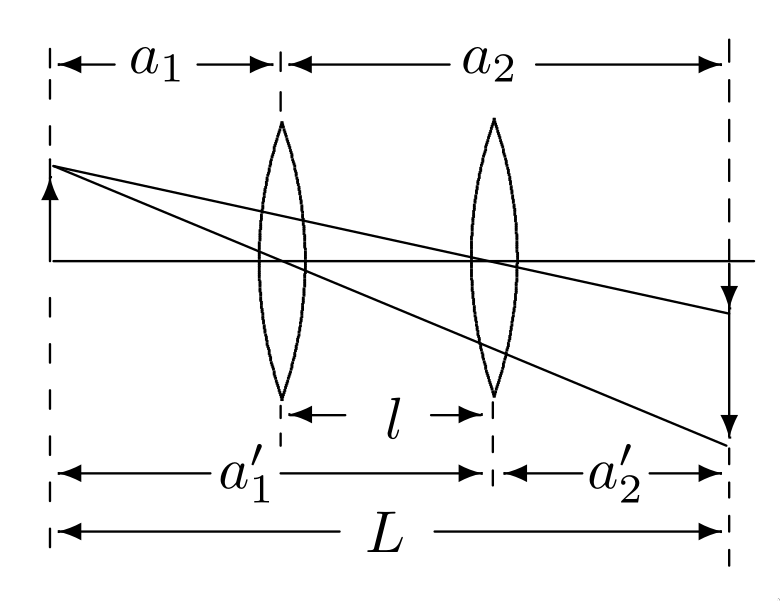
\includegraphics[scale=0.3]{pic_1.png}
    \caption{Схема измерения фокуса тонкой собирающей линзы}
\end{figure}

\noindent
Также фокусное расстояние тонкой собирабщей линзы можно измерить с помощью зрительной трубы, настроенной на бесконечность. Если расположить линзу между предметом и трубой и найти четкое изображение предмета, то расстояние от линзы до предмета будет равно фокусному.

\noindent
Для определения расстояние тонкой рассеивающей линзы поспользуемся схемой на рис. 2 и формулой тонкой линзы. Также можно восползоваться зриетльной трубой, настроенной на бесконечность. Если расположить предмет у нее в фокусе, то изображение переместиться в бесконечность, что можно проверить с помощью зрительной трубы.

\begin{figure}[H]
    \centering
    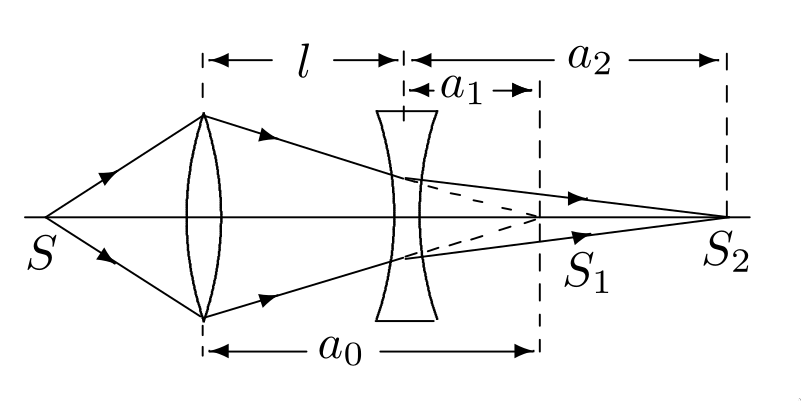
\includegraphics[scale=0.35]{pic_2.png}
    \caption{Схема измерения фокуса тонкой рассеивающей линзы}
\end{figure}

\noindent
Для определения фокусного расстояние и положения главных плоскостей сложной оптической системы может использоваться метод Аббе: схема на рис. 3 и формула (3).

\begin{figure}[H]
    \centering
    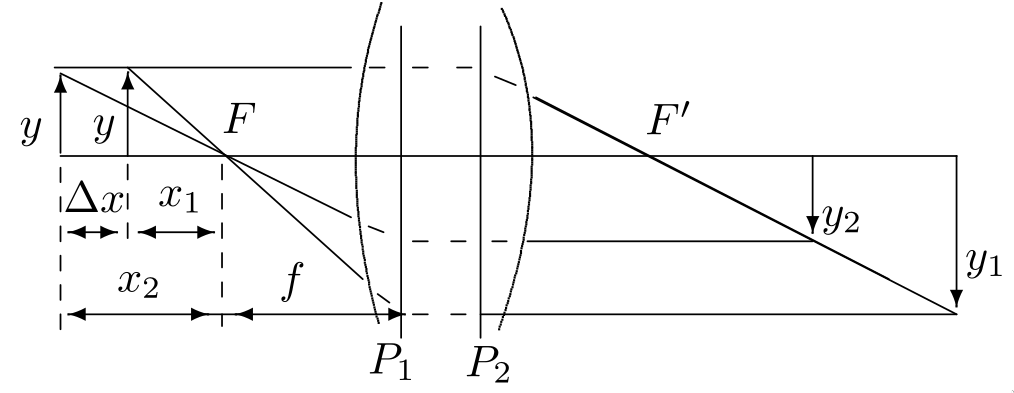
\includegraphics[scale=0.3]{pic_3.png}
    \caption{Схема определения фокусного расстояние и положения главных плоскостей сложной оптической}
\end{figure}

\begin{equation}
    f = \frac{\Delta x}{y / y_1 - y / y_2}
\end{equation}

Пусть пучок света, попадающий в объектив, составляет с оптической осью угол $\varphi_1$, а пучок, выходящий из окуляра, — угол $\varphi_2$. Увеличение $\gamma$ зрительной трубы по определению равно
\begin{equation}
    \gamma = \frac{\tan \varphi_2}{\tan \varphi_1},
\end{equation}
но также из рис. 3 следует, что
\begin{equation}
    \gamma_K = \frac{f_1}{f_2} = \frac{D_1}{D_2},
\end{equation}
где $D_1$ - ширина пучка, прошедшего через объектив, а $D_2$ - ширина пучка, вышедшего из окуляра

\subsection{Моделирование трубы Галилея}

    \begin{figure}[H]
    \centering
    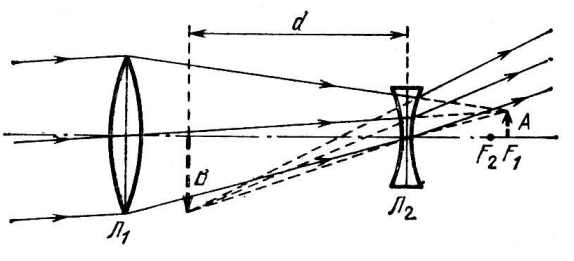
\includegraphics[width=9cm]{gal.PNG}
    \caption{Ход лучей в трубе Галилея}
    \label{fig:vac}
\end{figure}

\subsection{Моделирование микроскопа}

    \begin{figure}[h]
    \centering
    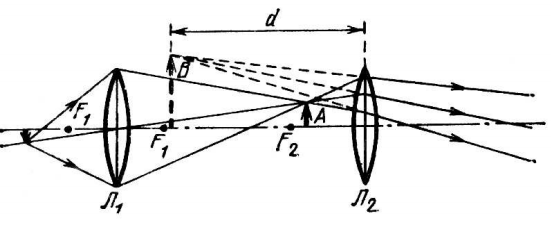
\includegraphics[width=9cm]{micro.PNG}
    \caption{Ход лучей в микроскопе}
    \label{fig:vac}
\end{figure}


Ход лучей в микроскопе показан на рис. 6. Увеличение микроскопа вычисляется по формуле
    \begin{equation}
        \gamma_M = \Gamma_{o_b} \Gamma_{o_c} = \frac{\triangle}{f_1} \frac{L}{f_2},
    \end{equation}.

    \begin{figure}[h]
    \centering
    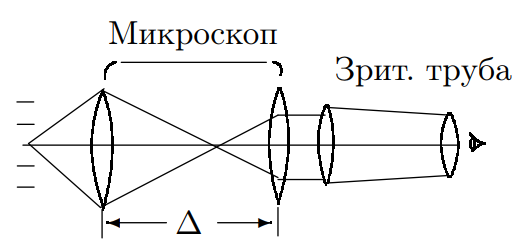
\includegraphics[width=9cm]{micro_2.PNG}
    \caption{Схема микроскопа}
    \label{fig:vac}
\end{figure}


\newpage
\section{Ход работы}
\subsection{Подготовка к работе}
%\par Работал я за установкой №3. Визуально определим, какие линзы являются собирающими, а какие -- рассеивающими. Собирающие линзы: 1, 2, 3, 4; рассеивающая линза: 5. Откорректируем высоту линз. Линза 1 не опускается ниже определённого уровня, так что использовать её далее мы не будем.
\par Определим фокусные расстояния линз с помощью экрана. С помощью формулы тонкой линзы подбирая расстояния между экраном, линзой и источникм, находим оценочные фокусные расстояния линз. Для нахождения фокусного расстояния рассеивающей линзы, поставим вплотную к ней собирающую, оптическая сила будет суммой сил каждой из линз. %Тогда получаем

% \begin{table}[h!]
% \centering
% \begin{tabular}{|l|l|l|l|}
% \hline
% $F_2$, см  & $F_3$, см & $F_4$, см  & $F_5$, см  \\ \hline
% 16 & 20 & 30 & -10 \\ \hline
% \end{tabular}
% \end{table}

\subsection{ Определение фокусных расстояний линз с помощью зрительной трубы}

Так как мы настроили зрительную трубу на бесконечность, то, если линза будет находится ровно на фокусном расстоянии от источника, то глядя в трубу мы будем видеть четкое изображение.

Для нахождения фокусного расстояние отрицательной линзы так же воспользуемся вспомогательной положительной, создавая для отрицательной линзы мнимый источник. Тогда фокусное расстояние отрицательной линзы будет $f = a_0 - l$


\begin{figure}[h]
    \centering
    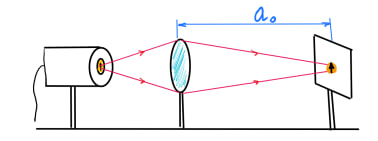
\includegraphics[width=9cm]{d1.jpg}
    \label{fig:vac}
\end{figure}

\begin{figure}[h!]
    \centering
    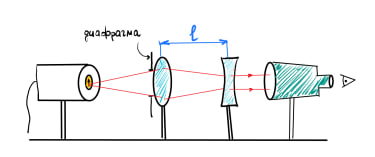
\includegraphics[width=9cm]{d2.jpg}
    \label{fig:vac}
\end{figure}

% \begin{table}[h!]
%     \centering
%     \begin{tabular}{|l|l|l|l|}
%     \hline
%     $F_2$, см  & $F_3$, см & $F_4$, см  & $F_5$, см  \\ \hline
%     14.9 & 19.4 & 29.6 & -11.5 \\ \hline
%     \end{tabular}
% \end{table}
% Для оценки того, тонкие линзы или нет, развернем линзы на 180 градусов и посмотрим как изменится фокусное расстояние. В частности для линзы 4 получается $F_4 = 29.5 см$, поэтому в пределах прогрешности будем считать линзы тонкими.

% \subsection{Измерение фокусных расстояний линз по формуле тонкой линзы и
% методом Бесселя}

% Возьмем линзу 2. Поставим экран от источника на расстояние  порядка $1.2 \cdot 4 F_2 = 71.5$ см.
% Поместим линзу в 2 положения на расстояниях $s_1$ и $s_2$. Получаем $s_1 = 38.0$ см, $s_2 = 66.5$ см.
% \par Тогда $l = s_2 - s_1 = 28.5$ см

% \begin{figure}[h!]
%     \centering
%     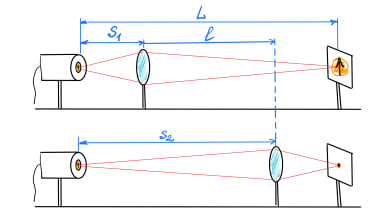
\includegraphics[width=9cm]{r.jpg}
%     \label{fig:vac}
% \end{figure}

% Тогда по приближенной формуле Бесселя:
% \begin{equation*}
%     f = \frac{L^2-l^2}{4L} = 15.0 \text{ см}
% \end{equation*}

% При переворачивании линзы получим точно такой же результат.



% \subsection{Измерение фокусных расстояний методом Аббе}

% Установим линзу 2 между осветителем и транспорантом в соответствии со схемой. В качестве физического предмета будем рассматривать изображение квадрата с линейным размером $y_0$.
% При изначальной установке размер изображения $y_1$. Отодвинем осветитель на некоторое расстояние $\Delta x = 4.8$ см от линзы. Затем передвинем экран к линзе на расстояние $\Delta x' = 15.9$ см до
% получения сфокусированного изображения с линейным размером $y_2$.

% \begin{table}[h!]
%     \centering
%     \begin{tabular}{|l|l|l|l|} \hline
%     $y_0$, см  & 0.5 & 1.3 & 1.9  \\ \hline
%     $y_1$, см  & 1.0 & 3.2 & 4.4  \\ \hline
%     $y_2$, см  & 0.5 & 1.7 & 2.4  \\ \hline
%     \end{tabular}
% \end{table}

% Тогда вычислить фокусное расстояние можно по формуле (возьмём размер большего квадратика для лучшей точности):

% \begin{equation*}
%     f = \frac{\Delta x'}{y_1/y_0 - y_2/y_0} = 15.1 \text{ см}
% \end{equation*}

% Или, если считать размер предмета неизвестным, то:

% \begin{equation*}
%     f^2 = \Delta x \cdot \Delta x' \cdot \frac{y_2y_1}{(y_2-y_1)^2} \quad \Rightarrow \quad f = 14.2 \text{ см}
% \end{equation*}

% \begin{figure}[H]
% 	\begin{minipage}[h]{0.5\linewidth}
% 		\center{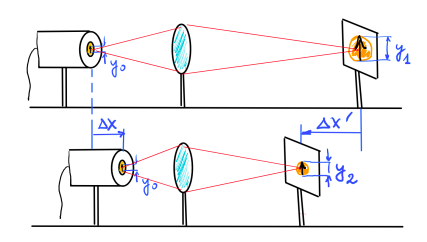
\includegraphics[width=0.95\linewidth]{ust3.png}}
% 	\end{minipage}
% 	\begin{minipage}[h]{0.5\linewidth}
% 		\center{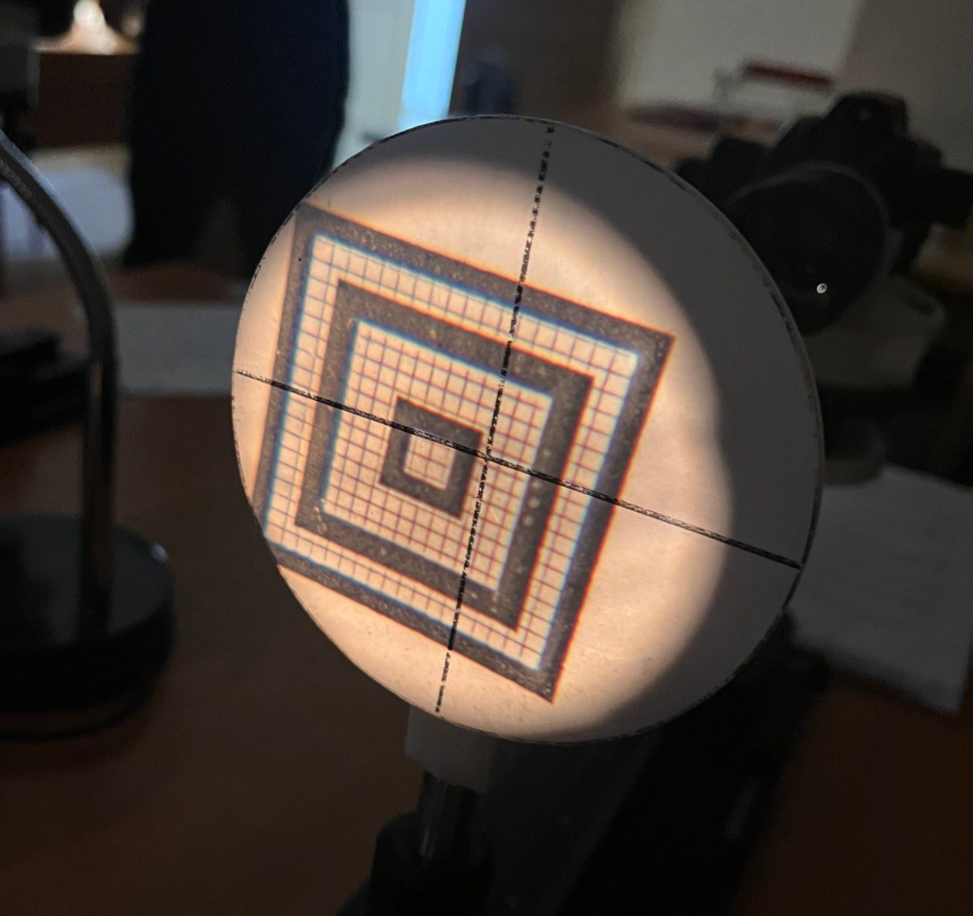
\includegraphics[width=0.9\linewidth]{qua2.png}}
% 	\end{minipage}
% \end{figure}


% \subsection{Сборка и изучение подзорной трубы Галилея}

% Сделаем подзорную трубу Галилея. Выберем 3 линзы: коллиматорную (4), объектив (2) и окуляр (5). Соберем модель телескопа Галилея

% \begin{figure}[h!]
%     \centering
%     \includegraphics[width=9cm]{photo_2024-04-08_23-08-57о.jpg}
%     \label{fig:vac}
% \end{figure}

% Соберём телескоп Галилея. Для этого для начала сымитируем удаленный объект. Для этого поставим длиннофокусную линзу и с помощью подзорной трубы, настроенной на бесконечность, найдем четкое изображение предмета.

% После определим угловой размер объекта $\alpha_0$ как кол-во рисок к числу укладывающихся периодов сетки (рис. \ref{pic:6}).

% \begin{figure}[h!]
%     \centering
%     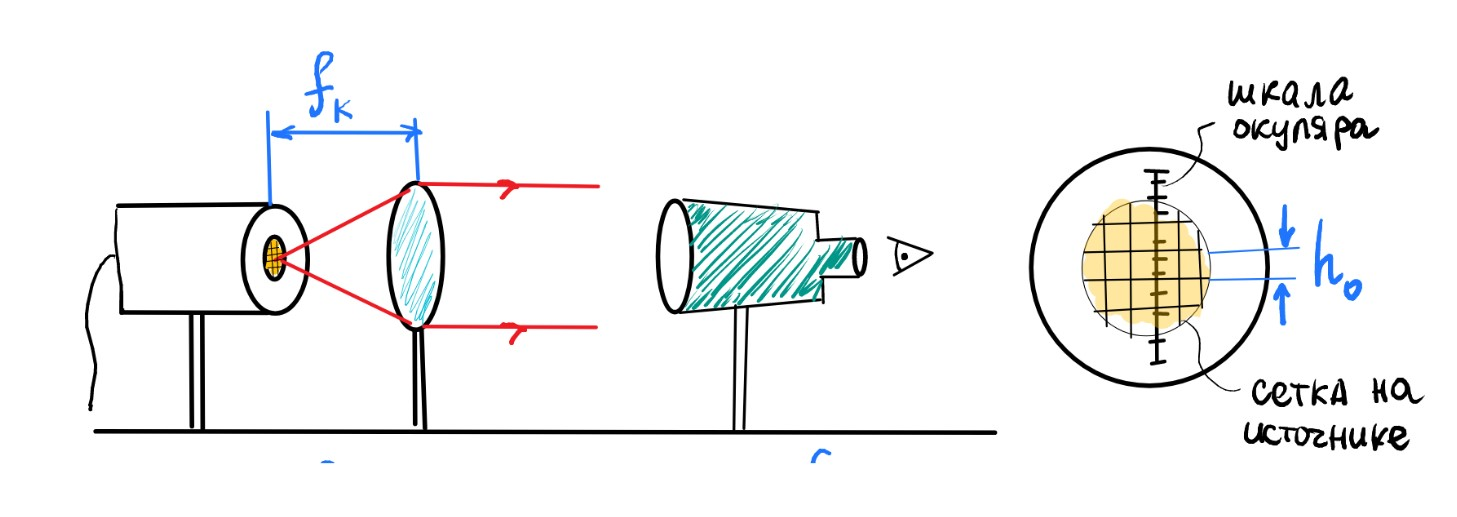
\includegraphics[width=9cm]{6.jpg}
%     \caption{Определение углового размера удалённого объекта}\label{pic:6}
% \end{figure}
% После начнем собирать телескоп. Для этого поставим две линзы $f_\text{ок}$ и $f_\text{об}$ (см. рис. \ref{pic:7}) и с помощью подзорной трубы, двигая окуляр, найдём четкое изображение сетки. После чего аналогичным способом (по кол-ву рисок к одному квадратику) определим угловой размер изображения $\alpha$ в телескопе. После посчитаем угловое увеличение телескопа $\gamma = \alpha / \alpha_0$. Теоретическое значение увеличения при этом равно $\gamma_\text{теор}= |f_\text{об} / f_\text{ок}|$.

% \begin{figure}[h!]
%     \centering
%     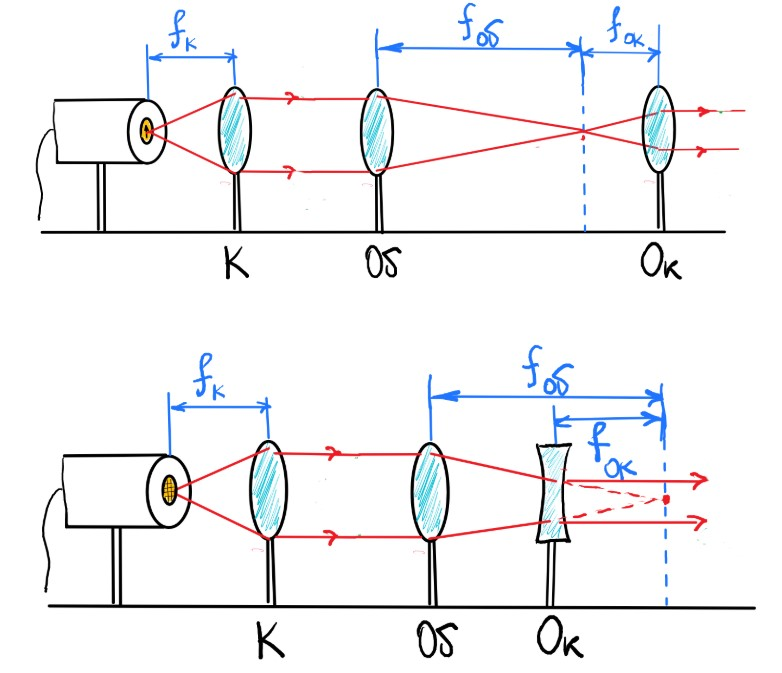
\includegraphics[width=9cm]{7.jpg}
%     \caption{Определение углового размера удалённого объекта в объективе телескопа}\label{pic:7}
% \end{figure}

% Также определить увеличение можно с помощью определения отношения диаметров изображения как $\gamma = D_\text{об} / D_\text{об}$ (см. рис. \ref{pic:8}).

% \begin{figure}[h!]
%     \centering
%     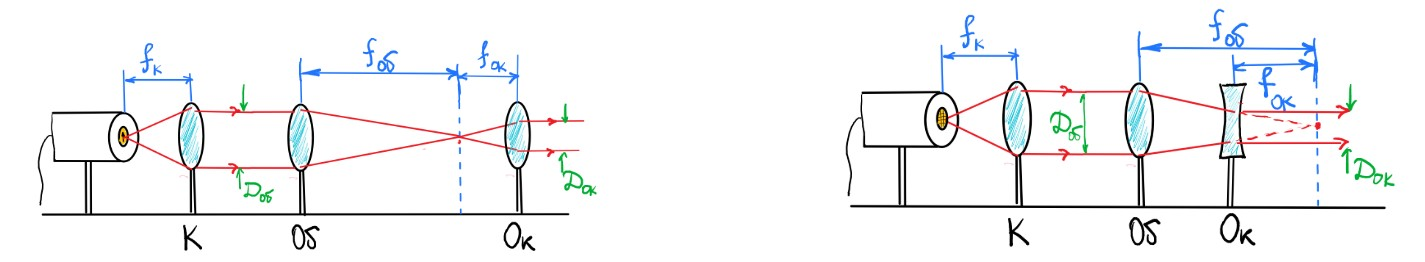
\includegraphics[width=18cm]{8.jpg}
%     \caption{Определение углового увеличения удалённого по размеру изображения}\label{pic:8}
% \end{figure}

% Коллиматор -- 300 мм, объектив -- 200 мм, окуляр -- 75 мм.  Получаем теоретическое увеличение $\gamma_\text{теор} = 2,66$. Посчитанное по кол-ву клеток в риске увеличение $\gamma = 2,8 \pm 0.4$ (погрешность большая, так как клетки были большими). Посчитанное с помощью размеров пятна $\gamma = 2.75 \pm 0.13$.

% \section{Вывод}

% Были исследованы различные способы нахождения фокусных расстояний линзы. Наиболее эффективным оказался метод с использованием подзорной трубы -- все значения совпали в пределах погрешности. Также неплохо показал себя метод Бесселя. Метод Аббе не получился из-за ошибки в выполнении.

% Также были собраны телескоп Кеплера и микроскоп и измерены их увеличения (только для телескопа).

% Также была изучена составная оптическая система. Найдены расстояния от линзы до фокальных плоскостей. Также с помощью метода Бесселя были найдены расстояния между фокусами линз и фокусное расстояние $F_2$.

% \begin{table}[h!]
% \begin{tabular}{|l|l|l|l|}
% \hline
% На глаз, см & Зрительная труба, см & Метод Бесселя, см & Метод Аббе, см \\ \hline
% 14.9       & 14.75                & 15.0         & 15.1      \\ \hline
% \end{tabular}
% \end{table}



\end{document}